\section{HPCG Test and Optimization}
This section focuses on the analysis and evaluation of HPCG. 
All the test results presented  are derived from the same hardware platform and software configuration for HPL, as detailed in Table \ref{tab:HPLHard} and Table \ref{tab:hpl software}.

\subsection{Analysis of HPCG}
\ 

The High Performance Conjugate Gradient (HPCG) benchmark is a key tool for assessing the performance of high-performance computing (HPC) systems, particularly in simulating real-world
computational workloads.
Unlike traditional benchmarks such as HPL, which mainly measure
floating-point operations through dense matrix multiplication, HPCG focuses on solving large sparse linear systems. 
These systems are derived from the discretization of a three-dimensional partial differential equation (PDE) that simulates a heat diffusion problem with zero Dirichlet boundary conditions.

At the heart of HPCG is the preconditioned conjugate gradient (PCG) method, which necessitates efficient handling of sparse matrix operations, optimized memory bandwidth, and parallel
computation across distributed systems. 
The global problem is defined on a three-dimensional grid
with dimensions $ (nx \times npx) \times (ny \times npy) \times (nz \times npz) $, where $nx$, $ny$, and $nz$ represent the local subgrid sizes in the $x$, $y$, and $z$ dimensions, respectively, assigned to each MPI process. 
The values $npx$, $npy$, and $npz$ denote the number of processes in each corresponding dimension. 
These values are automatically computed during the HPCG setup phase but can also be manually specified in the input file ``hpcg.dat" or provided as command-line arguments.

The HPCG benchmark consists of three critical computational kernels, each integral to evaluating modern supercomputer architectures:
\begin{enumerate}
    \item Sparse Matrix-Vector Multiplication (SpMV): The core computational task of HPCG, SpMV is computationally intensive and central to the benchmark’s performance evaluation.
    \item Symmetric Gauss-Seidel (SymGS) Relaxation: This serves as the essential preconditioning technique for the conjugate gradient method, enhancing the efficiency of the iterative solution process.
    \item  Conjugate Gradient Method: The iterative approach used to solve the large-scale sparse linear systems, making it a crucial component of HPCG’s overall performance.   
\end{enumerate}

These kernels are commonly found in scientific computing applications, such as computational fluid dynamics and electromagnetic simulations. 
They present significant challenges for system bandwidth and fine-grained parallel efficiency, making them indispensable for benchmarking modern HPC architectures.

\subsection{Performance Optimization Methods}
\ 

\subsubsection{Modification of ``HPCG.dat"}
\ 

By modifying the configuration parameters in the ``HPCG.dat" file, the optimization of the standard HPCG benchmark can be significantly impacted. 
The file contains two key sections that can be adjusted to improve performance: the problem size (specifically, the matrix size) and the runtime.
Adjusting the matrix size can have a major effect on performance.   

\begin{enumerate}
    \item \textbf{Matrix Size:} The matrix size defines the scale of the problem and is directly related to the global dimensions of the discretized computation grid. 
    By adjusting the local subgrid dimensions $(nx, ny, nz)$ and the number of subgrids in each dimension $(npx, npy, npz)$, the workload assigned to each MPI process can be optimized. 
    A larger matrix size generally increases computational complexity, which improves the scalability and performance of the benchmark on a large number of processors. 
    However, excessively large problem sizes may lead to memory limitations or imbalanced workload distribution between processes.
    Therefore, careful consideration of these parameters is essential for achieving optimal performance.
    \item \textbf{Runtime:} The runtime is another important parameter that influences the performance of the HPCG benchmark. 
    A longer runtime allows for more thorough testing of the system’s ability to handle sustained computational load. While a longer runtime provides a better measure of the system’s long-term stability and computing capacity, excessively long runtimes may lead to diminishing returns in performance due to hardware bottlenecks. 
    Therefore, choosing an appropriate runtime is essential to strike a balance between accuracy and benchmark duration. 
    In addition to the size of the topic scale, the shortest running time should be set to ensure the long enough running time of the system.
    Optimizing the matrix size and runtime in the ``HPCG.dat" file is crucial for fine-tuning benchmark performance, ensuring that the results reflect the system’s true capabilities.
    These modifications help with better load distribution, reduced memory overhead, and improved overall efficiency in parallel computing environments.
\end{enumerate}




\subsubsection{Third-Party Library for HPCG}
\ 

\begin{figure}[!htb]
    \centering
    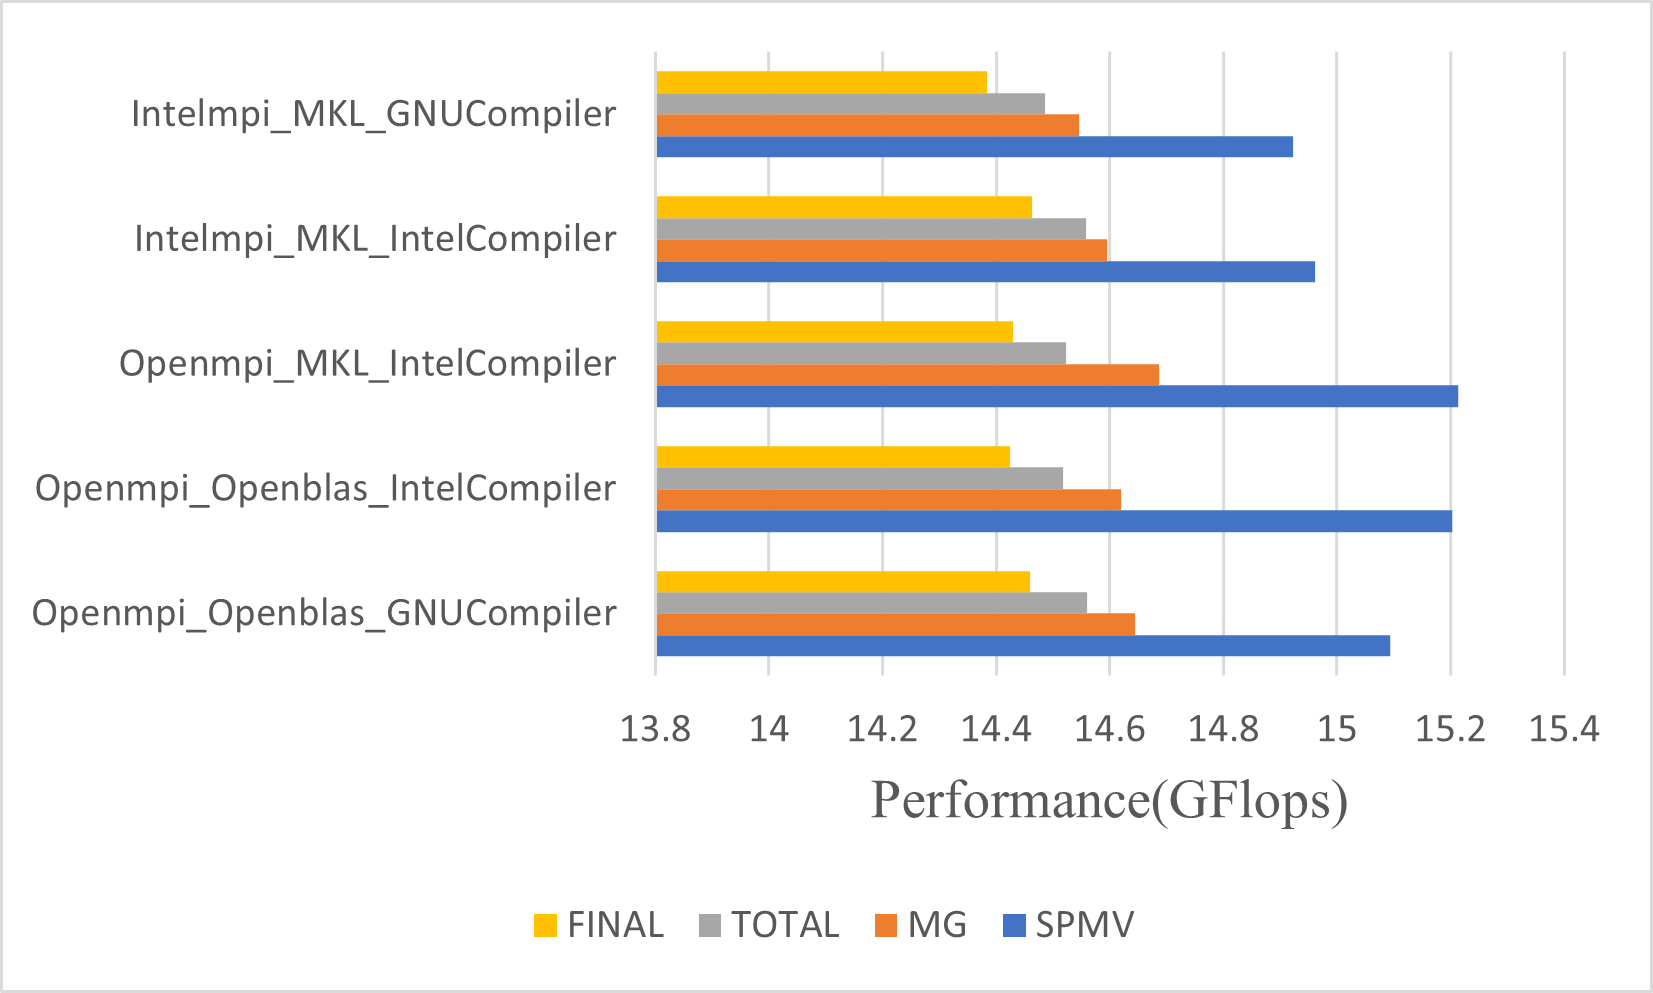
\includegraphics[width=0.8\linewidth]{figures/third party.png}
    \caption{Performance results for different third-party library settings in standard HPCG Benchmark}
    \label{fig:hpcg third party}
\end{figure}

For the standard HPCG benchmark, there are several third-party libraries available that can enhance performance. 
Key libraries include those for MPI and BLAS.
The commonly used MPI libraries are MPICH, OpenMPI, and Intel MPI (IMPI). 
These libraries handle the communication between different processes in a distributed computing environment.
For BLAS, several implementations are available, such as MKL (Intel Math Kernel Library), OpenBLAS, and Atlas.
BLAS libraries are crucial for performing optimized linear algebra operations on the CPU, which form a significant part of the HPCG computation.
After testing, we chose OpenBLAS and MKL as the BLAS libraries, while OpenMPI and Intel MPI were selected as the MPI libraries for communication.
The matrix size used in our experiments is set to $(160  \times 160  \times 128)$ and the runtime is fixed at 1800 seconds, which corresponds to the optimal parameter setting in Figure \ref{fig:hpcg third party}. 

% Please add the following required packages to your document preamble:
% \usepackage{subfig}



\subsubsection{Parallelization Paradigms for HPCG}
\ 

In this subsection, we explore three different configurations for the standard HPCG benchmark: MPI alone,  OpenMP alone, and  both MPI and OpenMP together. 
These configurations allow us to compare the performance of the standard HPCG benchmark under different parallelization paradigms and understand the impact of each parallelization method.
The matrix size used in our experiments is set to $(160  \times 160  \times 128)$, with the runtime fixed at
 1800 seconds. 
The third-party libraries used are OpenMPI and OpenBLAS, and the GNU Compiler is employed for compilation.

% Please add the following required packages to your document preamble:
% \usepackage{subfig}
\begin{figure}[!htb]
    \centering
    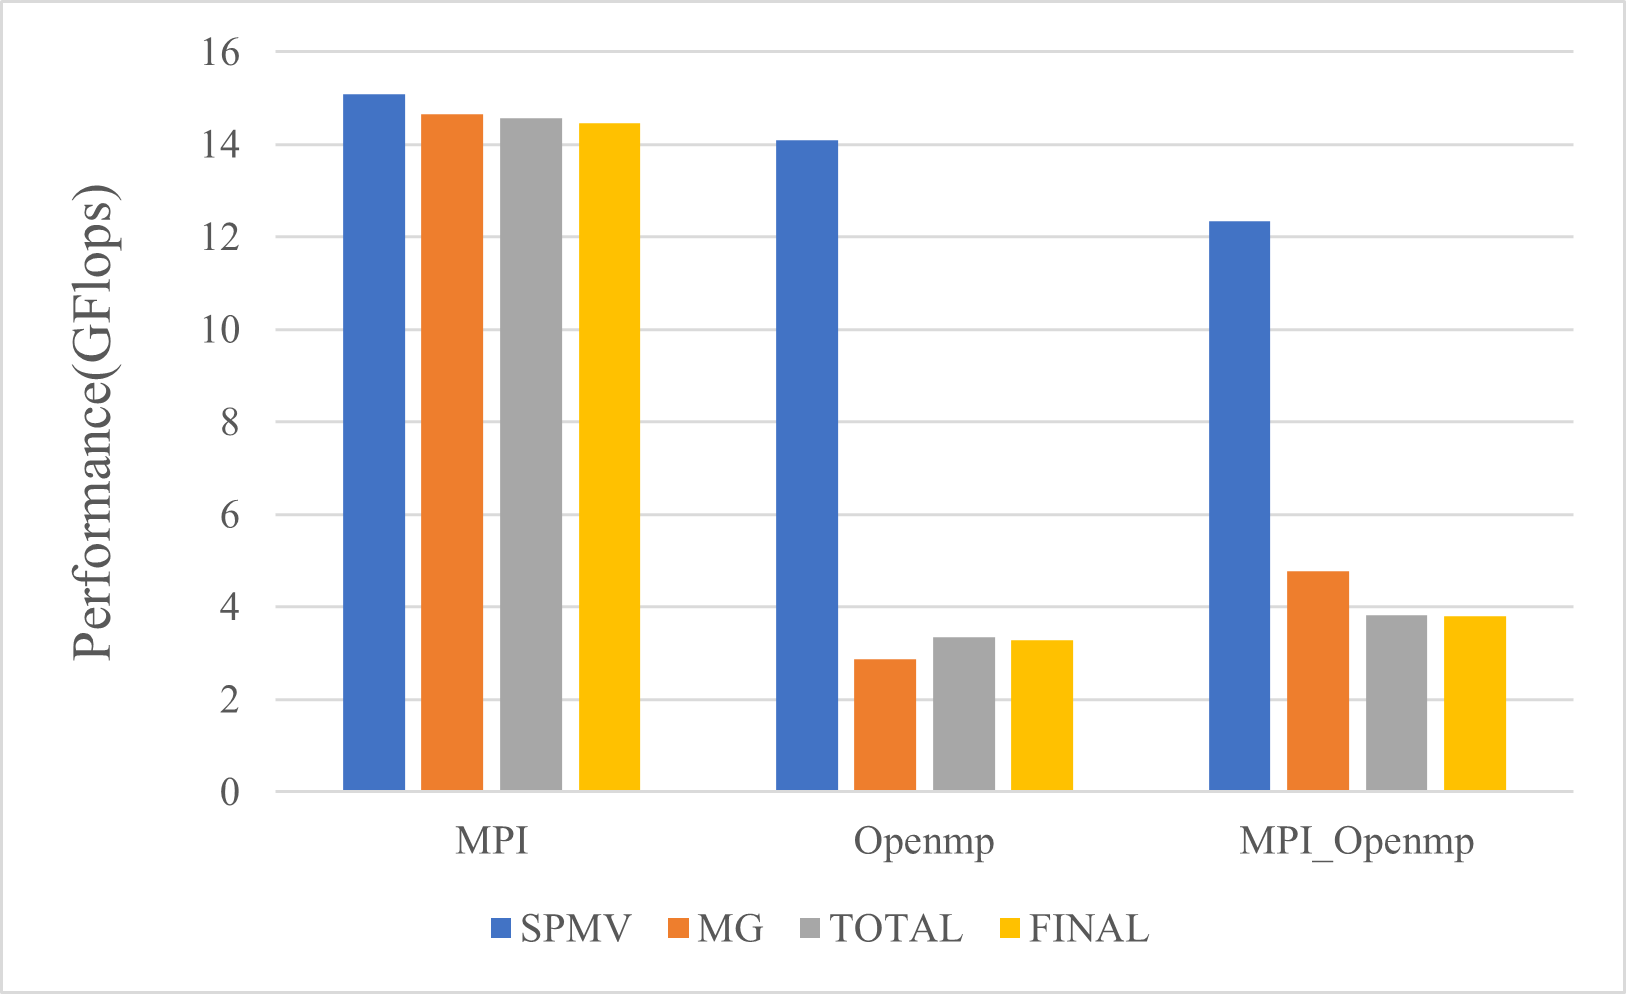
\includegraphics[width=0.8\linewidth]{figures/hpcg-mpi.png}
    \caption{Performance results for different Parallelization Paradigm settings in standard HPCG Benchmark}
    \label{fig:hpcg mpi}
\end{figure}

Based on the results of the experiments, as shown in Figure \ref{fig:hpcg mpi}, we observed that the configuration using MPI alone achieved the best performance across all tested machines. 
This configuration allowed the standard HPCG benchmark to fully utilize the distributed memory capabilities of the system, with each MPI process handling a portion of the problem.
The communication overhead, though present, was minimized due to the high efficiency of MPI in handling large-scale parallel problems.
In contrast, using OpenMP alone resulted in lower performance, primarily due to the limited scalability on a single-node setup. 
Although OpenMP effectively leveraged multicore CPUs, it was constrained by memory bandwidth and the relatively limited computational power available within a single node.
The hybrid  configuration performed well on multi-node systems, but the performance improvement was not as significant as expected. 
This is likely due to suboptimal load balancing between MPI and OpenMP, where the communication overhead between processes overshadowed the benefits of multi-threading within nodes. 
Moreover, hybrid configurations often require fine-tuning to achieve maximum performance, especially with larger problem sizes, which can result in a less straightforward optimization process.

\subsubsection{Hybrid Version of HPCG}
\ 

To further optimize performance, a hybrid approach can be applied to the HPCG benchmark, integrating CUDA for GPU acceleration. 
This allows the GPU’s floating-point performance to be exploited without altering the basic conjugate gradient (CG) algorithm or preconditioner algorithm.
The GPU’s parallel processing power is harnessed to significantly speed up matrix operations, which are a critical part of the HPCG benchmark.
In this hybrid version, the matrix is analyzed, reordered, and the computational workload is split between the CPU and GPU. 
The CPU handles portions of the matrix that are better suited for traditional processors, while the GPU is responsible for the portions that benefit most from parallel computation capabilities. 
This approach allows the hybrid version to capitalize on the strengths of both the CPU and GPU, optimizing performance for large-scale computations.
Fine-tuning the ratio of CPU to GPU workload is essential to achieve optimal performance. 
By experimenting with different configurations and workloads, the ideal distribution of tasks between
CPU and GPU can be found, maximizing the overall performance of the HPCG benchmark on systems equipped with both CPU and GPU resources.
The hybrid version allows HPCG to fully utilize both CPU and GPU resources, providing an effective solution for high-performance computing systems with multi-core CPUs and GPUs.


\subsection{Experimental Results}
\ 


\subsubsection{CPU Evaluation Results}
\ 

Since our server uses an AMD CPU, using the AMD-specific HPCG benchmark allows for the full utilization of its hardware features, resulting in a more accurate performance evaluation. 
Compared to the standard HPCG benchmark, the AMD version is optimized to better reflect performance in real-world applications. 
The following describes the test experiments for the AMD-specific
HPCG benchmark.
First, We conducted experiments by using only the CPU to run the AMD-specific HPCG benchmark. 
To achieve the best performance, we tested different data scales by adjusting the matrix size in the configuration file ``HPCG.dat".
By fine-tuning the matrix size, we sought to identify the optimal configuration for CPU-based computations on our AMD hardware.
And finally we get the best performance 21.2034 GFlops with:
\begin{itemize}
    \item \textbf{Matrix Size:} $512{\times}256{\times}256$.
    \item \textbf{Number of subgrids:} $npx{=}4$, $npy{=}2$, $npz{=}2$.
    \item \textbf{runtime:} 1800s.
\end{itemize}

So, the efficiency of the CPU evaluation is
\begin{equation}
    \text{Efficiency} {=}\frac{\text{Peak of HPL}}{\text{Theoretical Peak }} {=}\frac{\text{21.2034 GFlops}}{\text{947.2 GFlops }}{\approx}2.24\%
\end{equation}

\subsubsection{GPU Evaluation Results}
\ 

For GPU evaluation, we utilized the CUDA-enabled version of the HPCG benchmark.
The version we used is provided by NVIDIA and cannot be modified. Although we attempted to analyze the source code as time permitted, it is undeniable that there is a significant gap between our understanding and the optimizations implemented in the NVIDIA-provided version. 
Therefore, our current optimizations for HPCG were primarily achieved through parameter tuning in the ``HPCG.dat" file. 
These adjustments contributed to improved performance on GPU-based computations.
After testing multiple configurations, the optimal performance achieved was 232.673 GFlops with
\begin{itemize}
    \item \textbf{Matrix Size:} $256{\times}256{\times}256$.
    \item \textbf{Number of subgrids:} $npx{=}1$, $npy{=}1$, $npz{=}2$.
    \item \textbf{runtime:} 1800s.
    \item \textbf{Number of GPUs:} 2 (Dual GPU configuration).
\end{itemize}



\begin{equation}
    \text{Efficiency} {=}\frac{\text{Peak of HPL}}{\text{Theoretical Peak }} {=}\frac{\text{232.673 GFlops}}{\text{689 GFlops}\times 2}{\approx}16.88\%
\end{equation}

\subsection{Summary}
\ 

In the HPCG tests, our \textbf{CPU efficiency reached  21.2034 GFlops with  about 2.24\% efficiency}, and  \textbf{the GPU’s computational peak reaches 232.673 GFlops with about 16.88\% efficiency}.